%!TEX root = ../thesis.tex
%*******************************************************************************
%*********************************** Thrid Chapter *****************************
%*******************************************************************************

\chapter{Background Methodologies \label{cha:background}}  %Title of the Thrid Chapter

\nomenclature[a-GP]{$\mathcal{GP}\left(m(\cdot), k(\cdot, \cdot)\right)$}{Gaussian Process with mean function $m(\cdot)$ and covariance function $k(\cdot, \cdot)$}
\nomenclature[s-k]{$k$}{Principal component index.}

\ifpdf
    \graphicspath{{Chapter3/Figs/Raster/}{Chapter3/Figs/PDF/}{Chapter3/Figs/}}
\else
    \graphicspath{{Chapter3/Figs/Vector/}{Chapter3/Figs/}}
\fi

In the following chapter we consider the various statistical methodologies  upon which we build our CPACE model.
This chapter is structured as follows.
First we focus on common FDA techniques applicable to EO data.
We follow this by discussing smoothing methodologies which are of use in the FDA techniques. 
Finally we discuss Gaussian processes that are used in the CPACE framework to model correlation. 

\section{Functional Principal Components Analysis \label{sec:fpca}}
A commonly used technique in multivariate statistics is Principal Components Analysis (PCA), \citep{wold_principal_1987}. 
The technique finds dominant directions of variation and helps to achieve dimensionality reduction.
This offers a parsimonious way to view data which is driven by the data themselves.
The equivalent technique when the data are functional in nature is known as Functional Principal Components Analysis (FPCA), \citep{ramsay_functional_2010}.
The basic concepts were studied in the mid twentieth century.
The work of \citeauthor{karhunen_zur_1946} and independently \citeauthor{loeve_fonctions_1946} paved the basic foundations of the technique in the FDA literature, \citep{karhunen_zur_1946, loeve_fonctions_1946}.
The FPCA technique essentially stems from representing the random function $\mathcal{X}(t)$ as an infinite linear combination of orthogonal functions.
Such a representation is now known as the Karhunen-Lo\`{e}ve theorem after its discoverers.

\subsection{Formulation}
The formulation of FPCA begins by assuming that $\mathcal{X}(t)$, $t \in \mathcal{T}$ is a square integrable stochastic process over some domain $\mathcal{T}$.
By square integrable we formally mean that:

\begin{equation}
	\mathcal{X} \text{is square integrable} \iff \int_{\mathcal{T}} \lvert \mathcal{X}(t) \rvert^2 dt < \infty
\end{equation}

Let the mean and the covariance of the stochastic process $\mathcal{X}$ be denoted by $\mu(t)$ and $G\left(s, t\right)$ respectively, where:
\begin{align}
	\mu(t) &= \E \left(\mathcal{X}(t)\right) \label{eqn:mean_fn}\\
	G\left(s, t\right) &= \text{Cov}\left(\mathcal{X}(s),  \mathcal{X}(t)\right) \label{eqn:cov_fn}
\end{align}

Associated with the covariance surface $G\left(s, t\right)$ we have the linear operator $T_G$ defined by:
\begin{align}
	T_G &: L^2\left(\mathcal{T}\right) \to L^2\left(\mathcal{T}\right) \\
	T_G&:  f \mapsto T_G f = \int_{\mathcal{T}} G\left(s, \cdot \right) f(s) ds \label{eqn:t_op}
\end{align}
where $ L^2\left(\mathcal{T}\right)$ is the set of all square integrable functions over our domain $\mathcal{T}$. 

As $T_G$ is a linear operator we can consider its eigenvalues and eigenfunctions which we will denote by $\lambda_k$ and $\phi_k$ respectively (following convention set out in \citep{yao_functional_2005}) for $k=1,2,\cdots$.
These are defined as the solutions to the Fredholm integral equations of the second kind, \citep{yao_functional_2005}: 

\begin{equation}\label{eqn:fredholm}
	\langle G(\cdot, t), \phi_k \rangle = \lambda_k \phi_k(t)
\end{equation}
where $\langle f, g \rangle = \int_{\mathcal{T}} f(s) g(s) ds$ is the inner product in the space $L^2(\mathcal{T})$. 
Then by the Karhunen-Lo\`{e}ve theorem one can express the centred process through the eigenvalues and eigenfunctions of the linear operator associated to the covariance surface, \citep{karhunen_zur_1946, loeve_fonctions_1946}.
That is:
\begin{equation}\label{eqn:fpca}
	\mathcal{X}(t) - \mu(t) = \sum_{k=1}^{\infty}\xi_k \phi_k(t)
\end{equation}
where $\xi_k$ is the $k^\text{th}$ principal component associated to the eigenfunction $\phi_k$.
The Karhunen-Lo\`{e}ve theorem assures us this $L^2$ convergence is uniform in $t$.
The principal components are given by the following: 
\begin{equation}\label{eqn:principal_comp}
	\xi_k= \langle \mathcal{X} - \mu, \phi_k \rangle 
\end{equation}

Further to this decomposition the Karhunen-Lo\`{e}ve theorem means that the principal components are independent from each other, centred, and have variance equal to their associated eigenvalue, \citep{karhunen_zur_1946, loeve_fonctions_1946}.
That is:
\begin{align}
	\E\left(\xi_k\right) &= 0 \\
	\text{Var}\left(\xi_k\right) &= \lambda_k \\
	\E\left(\xi_k \xi_l\right) &= 0,~\text{for}~ k \ne l \label{eqn:principal_comp_uncorr}
\end{align}

\subsection{Interpretation}
As with the multivariate principal components analysis the interpretation of the eigenvectors is often useful in exploratory analysis of data.
The functional principal components analysis is of a similar form to the multivariate case and as such the same interpretation of the eigenfunctions is often employed.
The first eigenfunction $\phi_1(t)$ encapsulates the dominant mode of variation in $\mathcal{X}(t)$ by construction since:
\begin{equation}\label{eqn:first_comp}
	\phi_1 = \argmax_{\lVert \phi \rVert=1} \text{Var}\left( \langle  \mathcal{X} - \mu, \phi \rangle  \right)
\end{equation}
Similarly, the $k^\text{th}$ eigenfunction is the dominant mode of variation which is orthogonal to the preceding $k-1$ components.
Therefore exploring the first few eigenfunctions often gives a parsimonious way to view the variation in the data.
Alike multivariate PCA, it is often that the structure of the eigenfunctions replicates some observed physical process.
As such, the FPCA decomposition is often used widely as a tool for data exploration. 

In addition to this, we can use the fact that subsequent eigenfunctions capture less and less variation of the data as a form of dimensionality reduction, like PCA, \citep{wold_principal_1987}.
In this sense we can consider truncating the full representation given in Equation~\eqref{eqn:fpca} to the $K$ leading eigenfunctions which gives an approximation to the full process which we will denote by $\mathcal{X}^K(t)$ where:
\begin{equation}\label{eqn:fpca_trun}
	\mathcal{X}^K(t)  =   \mu(t) + \sum_{k=1}^{K}\xi_k \phi_k(t)
\end{equation}
The approximation of $\mathcal{X}$ by $\mathcal{X}^K$ converges as:
\begin{equation}\label{eqn:fpca_trun_conv}
	\E \left( \langle  \mathcal{X} - \mathcal{X}^K, \mathcal{X} - \mathcal{X}^K \rangle \right)  =   \sum_{k > K}^{\infty} \lambda_k \to 0~\text{as}~K \to \infty
\end{equation}

Using the leading principal components for reconstruction has the effect of capturing the main modes of variation of the data and ignoring smaller modes of variation.
Choosing the number of principal components is then up to the practitioner; as in multivariate PCA, \citep{wold_principal_1987}.
 \citeauthor{ramsay_functional_2010} discuss in length the comparison of PCA to FPCA including commentary on the optimal choice of the number of principal components, \cite[Chapter~8]{ramsay_functional_2010}.
 The practical implementation of FPCA then involves estimating various components.
 In particular estimation of;  the mean function $\mu(t)$, the covariance surface $G\left(s,t \right)$, the $K$ eigenfunctions and eigenvalues $\phi_k(t)$, $\lambda_k$ respectively, and the principal components $\xi_k$ for each realisation of the process $\mathcal{X}$ we observe.

\section{Principal Analysis Through Conditional Expectation \label{sec:pace}}
We will assume for now that we have a sufficient method for estimating the mean  and covariance surfaces which we will denote by $\hat{\mu}(t)$ and $\hat{G}\left(s, t \right)$ respectively.
We discuss in more detail the estimation of these components in Section~\ref{sec:splines}.
Prior to the introduction of the Principal Analysis through Conditional Expectation (PACE) methodology in \citep{yao_functional_2005} FPCA decomposition was restricted due to the need for approximating the integrals in Equation~\eqref{eqn:principal_comp}.
As such, it was often a requirement that the functional data were observed on a dense regular grid which meant that the principal components could be reliably estimated though some numerical integration scheme, \citep[Chapter~8]{ramsay_functional_2010}.
This very much restricted the application of the FPCA technique.
However \citeauthor{yao_functional_2005} introduced the PACE method for overcoming such an obstacle using conditional expectations for sparsely observed functional data, \citep{yao_functional_2005}.
At the same time the technique of \citep{yao_functional_2005} accommodates for observation error. 

Traditionally Equation~\eqref{eqn:principal_comp}, used for estimating the principal component scores for the $i^\text{th}$ realisation, is approximated through sums.
Substituting $y_{ij}$ for $\mathcal{X}(t_{ij})$, $\hat{\mu}(t_{ij})$ for $\mu(t_{ij})$, and $\hat{\phi}_k(t_{ij})$ for  $\phi_k(t_{ij})$ we obtain the estimate $\xi_i^{S} = \sum_1^{J_i}\left(y_{ij} - \hat{\mu}(t_{ij})\right)\hat{\phi}_k(t_{ij})\left(t_{ij} - t_{i(j-1)}\right)$, \citep{yao_functional_2005}, where $y_{ij}$ is as described in Equation~\eqref{eqn:fd_temporal} and setting $t_{i0}=0$.
However, such an estimate breaks for the case that observations are sparse.
Similarly this approximation will be biased when the error processes from Equation~\eqref{eqn:fd_temporal}, $\varepsilon_{ij}$, is non-zero.
\citeauthor{yao_functional_2005} overcome this by first assuming that the model is as follows, \citep{yao_functional_2005}:

\begin{align}
	y_{ij} &= \chi_{i}(t_{ij}) + \varepsilon_{ij} \\
	&= \mu(t_{ij}) + \sum_{k=1}^{\infty} \xi_{ik} \phi_k(t_{ij}) + \varepsilon_{ij} \label{eqn:fd_temporal_fpca}
\end{align}
with $\varepsilon_{ij}$ being jointly Gaussian with $\xi_{ik}$.
We also require the noise process satisfies:
\begin{align}
	\E\left(\varepsilon_{ij}\right) &= 0 \\
	\text{Var}\left( \varepsilon_{ij} \right) &= \sigma_\varepsilon^2
\end{align}

The number of measurements of the $i^\text{th}$ subject is considered random which reflect sparse functional data.
Such a description follows naturally from our dataset description, given in Equation~\eqref{eqn:fd_temporal}, by using the FPCA decomposition structure of $\mathcal{X}$ as discussed in Section~\ref{sec:fpca}.
Following \citep{yao_functional_2005} we define the subsequent vector notations:
\begin{align}
	\vesub{Y}{i} &= \left(y_{i1}, y_{i2}, \cdots, y_{iJ_i}\right)^\top \label{eqn:yvec}\\
	\vesub{\phi}{ik} &= \left(\phi_{k}(t_{i1}), \phi_{k}(t_{i2}), \cdots, \phi_k(t_{iJ_i}) \right)^\top \label{eqn:phivec} \\
	\vesub{\mu}{i} &= \left(\mu(t_{i1}), \mu(t_{i2}), \cdots, \mu(t_{iJ_i})\right)^\top \label{eqn:muvec}\\
	\vesub{t}{i} &= \left( t_{i1}, t_{i2}, \cdots, t_{iJ_i} \right)^\top \label{eqn:tvec}
\end{align}
With such a model and assumptions, as stated in \citep{yao_functional_2005}, the best prediction of the principal component scores for the $i^\text{th}$  subject is given by:
\begin{equation}\label{eqn:fpc_best}
	\tilde{\xi}_{ik} = \E\left(\xi_{ik} | \vesub{Y}{i}, \vesub{t}{i} \right) = \lambda_k \vess{\phi}{ik}{\top} \vess{\Sigma}{\vesub{Y}{i}}{-1} \left( \vesub{Y}{i} - \vesub{\mu}{i} \right)
\end{equation}
where $\vesub{\Sigma}{\vesub{Y}{i}} = \text{Cov}\left(\vesub{Y}{i}, \vesub{Y}{i} \right)$.
The estimate for the principal component score can then be found by substituting in estimates for the various components in Equation~\eqref{eqn:fpc_best}.
That is:
\begin{equation}\label{eqn:fpc_est}
	\hat{\xi}_{ik}= \hat{\E}\left(\xi_{ik} | \vesub{Y}{i}, \vesub{t}{i} \right) = \hat\lambda_k \hvess{\phi}{ik}{\top} \hvess{\Sigma}{\vesub{Y}{i}}{-1} \left( \vesub{Y}{i} - \hvesub{\mu}{i} \right)
\end{equation}
The covariance matrix $\hvesub{\Sigma}{\vesub{Y}{i}}$ is formed with $\left(l, m\right)^\text{th}$ element:
\begin{equation}\label{eqn:sig_cov}
	\left[\hvesub{\Sigma}{\vesub{Y}{i}}\right]_{lm} = \hat{G}(t_{il}, t_{im}) + \hat{\sigma}_\varepsilon^2 \delta_{lm}
\end{equation}
where $\hat{\sigma}_\varepsilon^2$ is the estimated variance of the noise process.
The estimation method for this is discussed in Section~\ref{sec:splines}.
\citeauthor{yao_functional_2005} also provide asymptotic properties of such an estimator  along with asymptotic confidence bands where the mean and covariance surfaces are estimated with local linear smoothers, \citep{fan_study_1996}.

The conditional expectation technique describe above from \citep{yao_functional_2005} alleviates the issue of poor integral approximation from sparsely observed data when the estimated covariance surface is a relatively good fit to the true covariance surface.
This is a somewhat better condition as it allows one to pool data from different observed subjects to estimate such a surface and thus the requirement of dense data per subject is relaxed to having dense data from the collection over all subjects.
We discuss a particular method for estimating such surfaces in Section~\ref{sec:splines}.

\section{Penalised Regression Splines \label{sec:splines}}
 Smoothing models underpin much of FDA.
 FDA uses the smoothness of observations over a continuous domain to help inform and model observed data, \citep{ramsay_functional_2010}.
 Typically, as described in Section~\ref{sec:fr}, data is only observed discretely.
 Therefore with most FDA methodology there must be a conversion from discretely observed data and the continuous functional variable that generates it.
 This is particularly the case for our EO data since we have discrete observations specified by our data model given in Equation~\eqref{eqn:observed_data} which we assume is generated by observations of continuous functions given by our models in Equation~\eqref{eqn:fd_temporal}.
 Many models for obtaining a smooth of the data have been studied, such as kernel smoothing, polynomial regression, and local linear smoothing, \citep[Chapter~4]{ramsay_functional_2010}. 
 In this section we consider the well studied technique of obtaining smooths of discrete data through penalised regression splines, \citep{ruppert_semiparametric_2003}.
 We will use such a method to estimate the mean and covariance surfaces present in the PACE methodology as described in Section~\ref{sec:pace}. 
 We first describe the components that form the foundations of a regression spline; the spline basis.
 
 \subsection{Basis splines  \label{ssec:basis_splines}}
 One of the components of a penalised regression splines is the basis functions used in the regression.
 As the name suggests regression splines uses spline functions as the regression basis.
 A spline function of order $d$,  which is well documented in the monograph of \citeauthor{de_boor_practical_2001}, is a piecewise polynomial function of degree $d-1$, \cite{de_boor_practical_2001}.
 In the case of a spline function of order $d$ over a univariate domain $\mathcal{T} = \left[a, b\right] \subset \mathbb{R}$, which we denote by $S: \mathcal{T} \to \mathbb{R}$,  we have: 
 \begin{equation}
 	S: t \mapsto S(t) = \begin{cases}
 		P_0(t)~\text{if}~ \tau_0 < t  \leq \tau_1,\\
 		P_1(t)~\text{if}~ \tau_1 < t  \leq \tau_2,\\
 		\vdots \\
 		P_{m-1}(t)~\text{if}~ \tau_{m-1} < t  \leq \tau_m,\\
 	\end{cases}
 \end{equation}
where $P_i: \left[\tau_i, \tau_{i+1}\right] \to \mathbb{R}$ are polynomial functions of degree $d-1$.
The vector of points $\ve{\tau} = \left(\tau_0, \tau_1, \cdots, \tau_m \right)$ is known as the knot vector for the spline and must satisfy $a=\tau_0 < \tau_1 < \cdots < \tau_m = b$.
By specifying that the piecewise polynomials must share the same derivative order up to a degree we can ensure continuity of relative smoothness over the knot points and the whole spline function.
We specify the continuity at each point in our knot vector by the continuity vector $\ve{r}=\left( r_0,\cdots, r_m \right)^\top$ where $r_i$ specifies that $P_i$ and $P_{i+1}$ share common derivative values at point $\tau_i$ for derivatives up to order $r_i$.
The spline type can be specified completely by specifying the knot locations and the continuity vector, \citep{de_boor_practical_2001}.
In fact, one can extend our definition of the knot vector to incorporate both the knot and continuity vector into one.
This is known as the extended knot vector, which will completely specify the spline type, \citep{de_boor_practical_2001}.
We define the extended knot vector as the vector of knot points which repeats the $i^\text{th}$ knot vector exactly $n - r_i$ times. That is:
\begin{equation*}
	(\tau_0,\cdots,\tau_0, \tau_1, \cdots, \tau_1 ,\cdots, \tau_{m-1},\cdots, \tau_{m-1}, \tau_m \cdots, \tau_m)
\end{equation*}
We denote the spline functions of order $d$ with extended knot vector by $S_{d, \ve{\tau}}$. 

The Basis splines are more commonly referred to as B-splines, \citep{knott_interpolating_2000}.
B-splines are basis functions for splines of the same order defined over the same knots.
They are typically defined recursively, \citep{knott_interpolating_2000, de_boor_practical_2001}.
The classic algorithm for the recursive construction is known as the Cox-de Boor recursion formula, \citep{de_boor_practical_2001}, and is given as follows.
Given a knot vector $(\tau_0,\cdots,\tau_0, \tau_1,\cdots,  \tau_1, \cdots, \tau_{m-1},\cdots, \tau_{m-1}, \tau_m,\cdots, \tau_m)^\top$ the B-spline of order $1$ is given by:
\begin{equation}	\label{eqn:bspline1}
	B_{i, 1}\left( t \right) = \begin{cases} 1,~\text{for}~\tau_i \le t < \tau_{i+1} \\ 0,~\text{otherwise.} \end{cases}
\end{equation}

The higher order B-splines are defined by recursion as:
\begin{equation}\label{eqn:bspline_high}
	B_{i, q+1}(t) = w_{i, p}(t) B_{i, q}(t) + \left[ 1 - w_{i+1, q}(t) \right]B_{i+1, q}(t)
\end{equation}
where $w_{i, q}$ is a weighting for the $i^\text{th}$ B-spline of order $d$ given by:
\begin{equation}
	w_{i, q}(t) = \begin{cases} \frac{x-\tau_i}{\tau_{i+q} - \tau_i} ,~\text{for}~\tau_{i+q} \ne \tau_i \\ 0,~\text{otherwise.} \end{cases}
	\label{eqn:weighting}
\end{equation}
A B-spline basis system of size $Q$ can then be considered by choosing the extended knot vector $\ve{\tau}$ and specifying the order, $d$, of the B-spline functions, and is given by the collection:
\begin{equation}
	\{ B_{d, q}^{\ve{\tau}}(t)\}_{q=1}^{Q}
	\label{eqn:bspline_basis}
\end{equation}
where $Q$ is the number of basis functions to use in the system, $\ve{\tau}$ is the extended knot vector, and $B_{d, q}^{\ve{\tau}}$ is the $q^\text{th}$ B-spline of order $d$ defined by Equation~\eqref{eqn:bspline_high} for our knot vector $\ve{\tau}$.

\subsection{Regression splines \label{ssec:spline_reg}}
As discussed in Section~\ref{sec:pace} the PACE methodology requires estimation of both the mean function, $\mu(t)$, and covariance surface $G\left(s, t\right)$. 
Estimating such functions is a problem due to their infinite dimensional nature.
A well studied and effective method for representing such functions is the use of a basis function expansion,  \cite{ramsay_functional_2010}.
That is representing the target surface using a linear combination of known basis functions.
In this work we will utilise the B-spline basis function; as discussed in Section~\ref{ssec:basis_splines}.
The B-spline system is exceptionally popular due to its ease of computation and ability to reconstruct many surfaces, \citep{de_boor_practical_2001}.
Such ease of computation makes it feasible to not only create large basis systems but also alleviates many fitting procedures as we can re-evaluate the basis system at various points with ease.
These properties are very useful when using such a basis for regression models. 
Other common basis systems include the Fourier, Monomial, and Polynomial basis systems.
See \citep{ramsay_functional_2010} for details of these basis systems in the functional framework.
In the following we present the approach for estimating an arbitrary realisation of our functional random variable $\chi_i(t)$ over domain $\mathcal{T}$ and discuss how we extend the same concept to a two dimensional surface over $\mathcal{T} \times \mathcal{T}$.

We assume that our function  can be represented using an order $d$ B-spline basis system with knot vector $\ve{\tau}$: 

\begin{align}
	\chi_i(t) &= \sum_{q=1}^Q c_q B_{d, q}^{\ve{\tau}}(t) \\
	&= \vesup{c}{\transpose} \vess{B}{d}{\ve{\tau}}(t) \label{eqn:basis_expansion}\\
\end{align}
where $\ve{c}=\left( c_1,\cdots, c_Q \right)^\transpose$, $\vess{B}{d}{\ve{\tau}}(t) = \left( B_{d, 1}^{\ve{\tau}}(t), B_{d, 2}^{\ve{\tau}}(t), \cdots, B_{d, Q}^{\ve{\tau}}(t) \right)$, and $Q$ is the dimension of the expansion.
If such basis functions have nice properties like being easy to compute then such a representation for $\chi_i$ given by Equation~\eqref{eqn:basis_expansion} can be extremely useful since most problems can be reduced to involving only the finite dimensional vector $\ve{c} \in \mathbb{R}^Q$. 

Our representation of $\chi_i$ using a basis system then becomes the problem of choosing the coefficients $\ve{c}$ using only our set of observations of $\vesub{Y}{i}$ which are observed with error.
The most common method for fitting a basis system to discretely observed data is by choosing the coefficients of the expansion, $c_q$, given in Equation~\eqref{eqn:basis_expansion} by minimising the criterion, \cite{bjorck_numerical_1996}:
\begin{equation}
	\text{SSE}_{\vesub{Y}{i}}\left( \ve{c}\right) = \lVert \vesub{Y}{i} - \ve{B}\ve{c} \rVert^2
	\label{eqn:sse}
\end{equation}
where $\ve{B} = \left( \vess{B}{d}{\ve{\tau}}(t_{i1}),\vess{B}{d}{\ve{\tau}}(t_{i2}),\cdots, \vess{B}{d}{\ve{\tau}}(t_{iJ_i}) \right)^\transpose$ is the $J_i \times Q$ matrix of the basis system evaluated at observed time points corresponding to the $J_i$ length observation vector $\vesub{Y}{i}$. Minimising such a criterion is given by, \cite{bjorck_numerical_1996}:
\begin{equation}
	\hat{\ve{c}} = \left( \vesup{B}{\transpose} \ve{B} \right)^{-1}\vesup{B}{\transpose}\vesub{Y}{i}
	\label{eqn:hatc}
\end{equation}

The simple least squares approximation is a well studied and standard approach.
See \citep{bjorck_numerical_1996} for a thorough introduction to the concept. 
Such a methodology is often suitable for situations where our error process $\varepsilon(t)$ is a white noise process.
This process for the noise is often unrealistic; as such a simple adjustment to the least squares criterion in Equation~\eqref{eqn:sse} can be used to allow for correlation among the observation errors: 
\begin{equation}
	\text{SSE}_{\vesub{Y}{i}, \ve{W}}(\ve{c}) = \lVert \ve{W}^\frac{1}{2}\left( \vesub{Y}{i} - \ve{B}\ve{c} \right) \rVert^2
	\label{eqn:wsse}
\end{equation}
where $\ve{W}$ is a weighting matrix for the observations. Ideally the matrix will be the inverse of the variance-covariance matrix of the observations. Minimising the adjusted criterion is given by, \cite{bjorck_numerical_1996}:
\begin{equation}
	\hat{\ve{c}} = \left( \vesup{B}{\transpose} \ve{W} \ve{B} \right)^{-1}\vesup{B}{\transpose} \ve{W} \vesub{Y}{i}
	\label{eqn:whatc}
\end{equation}
The estimate with least squares fitting can then be found by substituting $\hat{\ve{c}}$ for the $\ve{c}$ in Equation~\eqref{eqn:basis_expansion}, \citep{bjorck_numerical_1996}. That is:
\begin{equation}\label{eqn;hat_basis_expansion}
	\hat{\chi}_i(t) = \vesup{\hat{c}}{\transpose} \vess{B}{d}{\ve{\tau}}(t)
\end{equation}
The selection of the knot vector is well studied and the classical choice is to choose a knot vector where knots are located at the sampling points, \citep{de_boor_practical_2001}. 

An issue with the classical least squares fitting using a basis system expansion is the choice of number of basis functions, \cite{ramsay_functional_2010}.
We are constrained to choose $Q$ to be less than or equal to the number of observations, $J_i$. This is because more than $J_i$ basis functions would results in Equation~\eqref{eqn:whatc} being ill defined since the matrix $\ve{B}$ would have linearly dependent columns.
However, we still have the choice to choose $Q$ between $1$ and $J_i$.
Exactly which value for $Q$ to choose is unknown and results in bias - variance trade off in the estimator, \citep{ramsay_functional_2010}.
A large number of basis functions reduces bias in the estimator $\hat{\chi}_i(t)$, but the variance of this estimator may be unacceptably high.
Conversely, a lower number of basis functions will result in high bias of the estimator but low variance.
The bias-variance trade off is well studied and there is a vast literature on the methodology of choosing the number of basis functions. 
However, there is no gold standard and often the choice is made in an ad hoc fashion, \citep{ramsay_functional_2010}. 
Such an issue motivates modifying the fitting criterion which determines $\ve{\hat{c}}$ in Equation~\eqref{eqn:whatc}.

\subsubsection{Penalties}
Ideally, we want to penalise estimators which have high variance, that occur naturally when we have a large number of basis functions, but keep bias low.
The naive choice of just reducing the number of basis functions, known as regression splines,  fails in this respect, \citep{ruppert_semiparametric_2003}.
One such approach to do this is to reduce the number of basis functions in conjunction with a penalty, known as penalised regression splines, \citep{ruppert_semiparametric_2003}.
Such an approach was first used in \citep{osullivan_statistical_1986} who applied such a technique to ill posed inverse problems.
\citep{ruppert_semiparametric_2003} discusses various other spline smoothing techniques as well as the penalised regression splines.

Penalised regression spline models adjust the fitting criterion in Equation~\eqref{eqn:whatc} to, \citep{ruppert_semiparametric_2003}:
\begin{equation}\label{eqn:plss}
	\text{PSSE}_{\vesub{Y}{i}, \ve{W}, \lambda}(\ve{c}) = \lVert \vesup{W}{\frac{1}{2}}\left( \vesub{Y}{i} - \ve{B}\ve{c} \right) \rVert^2 + \omega \vesup{c}{\transpose} \ve{P} \ve{c}
\end{equation}
where $\ve{P}$ is formed with $(l,m)^\text{th}$ element $\left[\ve{P}\right]_{lm} = \langle L\left(\vesub{B}{l}\right), L\left( \vesub{B}{m} \right) \rangle$ and $\omega$ is a parameter which controls the regularisation trade off.
$L$ is some linear differential operator.
Typically, one chooses $L$ to be the required smoothness of the target function and examples include simple first or second derivatives, \cite{ruppert_semiparametric_2003}.

Analytically minimising the $\text{PSSE}$ criterion in Equation~\eqref{eqn:plss} can be found via, \citep{ruppert_semiparametric_2003}:
\begin{equation}
	\hat{\ve{c}} = \left( \vesup{B}{\transpose} \ve{W} \ve{B} + \omega \ve{P} \right)^{-1}\vesup{B}{\transpose} \ve{W} \vesub{Y}{i}
	\label{eqn:phatc}
\end{equation}

Essentially, such a penalisation term determines that there should be a trade off between the bias which corresponds to the first term in Equation~\eqref{eqn:plss} and the variance which is the second term.
This trade off is controlled by the regularisation parameter $\omega$.
The advantage of this method is that we can now let $Q$, our number of basis functions, be large without worrying of over fitting as the penalty term in Equation~\eqref{eqn:plss} will penalise functions with high variability in terms of the differential operator $L$.

The choice of differential operator is a well studied problem also. A common choice is the first or second order differential, denoted by  $D^1$ and  $D^2$ respectively, as this specifies a reasonable level of smoothness in the target function, \cite{ruppert_semiparametric_2003}.
However, often more complex terms are used to facilitate known properties of the target functions, such as letting $L$ be the harmonic acceleration operator which forces a periodic form of the target functions.
More care must be taken when extending the linear differential operator to higher dimensions which is discussed below.
Additionally, in the case of B-spline basis system these penalty matrices are typically evaluated using a form of numerical integration, \cite{ramsay_functional_2010}.

Penalised regression splines moves our problem of selecting $Q$ to choosing our regularisation parameter, $\omega$.
Such a parameter influences the strictness with which we expect our target function to be smooth as defined by the operator $L$.
Choosing this parameter is a problem that is present not only in spline smoothing but other penalised regression approaches, \citep{lukas_robust_2006}.
A popular method for choosing such a parameter is Generalised Cross Validation (GCV).
GCV, introduced by \citeauthor{wahba_practical_1977} in \citep{wahba_practical_1977}, is a well studied method which has good asymptotic properties as the number of observations tends to infinity, \citep{wahba_spline_1990, wahba_comparison_1985}.
GCV chooses $\omega$ as the minimiser of the GCV criterion $V(\omega)$ which is given by, \citep{wahba_spline_1990}:
\begin{equation}\label{eqn:gcv}
	V\left(\omega\right) = \frac{J_i^{-1} \lVert \left(\ve{I} - \ve{A} \right) \vesub{Y}{i} \rVert^2}{\left[ J_i^{-1} \text{tr}\left(\ve{I} - \ve{A}\right)\right]^2}
\end{equation}
where $\ve{A}$ is the influence matrix defined by:
\begin{equation}\label{eqn:inf}
	\ve{A} = \ve{B} \left( \vesup{B}{\transpose} \ve{W} \ve{B} + \omega \ve{P} \right)^{-1}\vesup{B}{\transpose} \ve{W}
\end{equation}
The GCV method can then be minimised for $\omega$ using a numerical minimisation routine.
For large $J_i$ it is known that the GCV criterion performs well in recovering a regularisation parameter which minimises variance while maintaining low bias in the reconstruction of the target function, \citep{wahba_comparison_1985}.
For the case of low $J_i$ the GCV method may not be reliable.
As such, methods to extend the GCV criterion have been considered.
The modified GCV criterion adds a further modifier to the denominator in Equation~\eqref{eqn:gcv} by multiplying the trace of the influence matrix by a factor, \citep{cummins_confidence_2001}.
The modified GCV approach effectively increases the cost associated with each effective parameter in the curve which reduces the chance of choosing an $\omega$ which under smooths the data, \citep{cummins_confidence_2001}.
A similar but separate approach to adjusting the GCV is robust GCV, introduced by \citeauthor{lukas_robust_2006}.
\citeauthor{lukas_robust_2006} uses a weighted sum of the GCV function with a term which penalises $\omega$ values that are close to zero, \citep{lukas_robust_2006}.
The performance of such methods are discussed in \citep{lukas_performance_2012}.

Choosing a basis system, a criterion to choose the regularisation parameter, and a differential operator then fully specifies the penalised regression spline approach.
In the case of one dimensional functions the procedure applies as above. As such, we can estimate our mean function $\mu(t)$ through the use of a penalised regression splines where our observation points for the mean function are the pooled mean across subjects of the union of observed time points for all curves.
However for multiple dimensions, particularly the case when we wish to smooth the covariance surface, we must make some adjustments to the approach described above.

\subsubsection{Extension to higher dimensions \label{sssec:spline_ext}}
There are two issues when extending the penalised regression spline to higher dimensions; extending the basis system and extending the penalty specification.
To alleviate the first we must specify a basis system which can cover multiple dimensions. In fact there are many such systems, \citep{wahba_spline_1990}.
One popular approach when we have regular data for FDA is using a tensor product B-spline system, \citep{xiao_asymptotic_2020}.
We describe the extension to two dimensional surfaces, but the same extension will work for higher dimensional surfaces.
Consider a two dimensional surface, $\sigma \left(s, t\right)$, which we represent by the tensor product spline given by, \citep{xiao_asymptotic_2020}:
\begin{equation}\label{eqn:tensor_expansion}
	\sigma \left(s,t\right) = \sum_{1 \le q_1, q_2 \le \bar{Q}} c_{q_1, q_2} \vess{B}{d_1}{\vesub{\tau}{1}}(s)\vess{B}{d_2}{\vesub{\tau}{2}}(t)
\end{equation} 
where $\vess{B}{d_i}{\vesub{\tau}{i}}$ is the B-spline basis system for the $i^\text{th}$ dimension for $i=1,2$.
For notational simplicity we assume the dimension of each marginal basis system is the same, $\bar{Q}$. 
However, in general this need not be the case.
$\ve{C} \in \mathbb{R}^{\bar{Q} \times \bar{Q}}$ is a coefficient matrix to be determined.
Equation~\eqref{eqn:tensor_expansion} can be written more succinctly using a Kronecker product as, \citep{xiao_asymptotic_2020}:
\begin{equation}\label{eqn:kron_expansion}
	\sigma\left(s,t\right) = \vesup{\bar{B}}{\transpose}\left(s, t\right) \text{Vec} \left(\ve{C}\right)
\end{equation}
where $ \ve{\bar{B}}\left(s, t\right) = \vess{B}{d_2}{\vesub{\tau}{2}}(t) \otimes \vess{B}{d_1}{\vesub{\tau}{1}}(s)$ and $\text{Vec}\left(\cdot\right)$ is an operator which stacks the columns of a matrix into a vector. We use the $\bar{\cdot}$ notation to make explicit that this basis is over multiple dimensions.

The same methods now follow as in the non penalised univariate case with this Kronecker basis system, \citep{xiao_asymptotic_2020}.
However, we must still adjust the penalty matrix in Equation~\eqref{eqn:phatc} to account for smoothness across multiple dimensions. 

Using the tensor product basis system as described above; one might consider specifying the smoothness of the function in each dimension.
Indeed, one such approach to extending the penalty specification which was introduced by \citeauthor{wood_low-rank_2006} is to consider setting penalties on the marginal basis separately and to combine them by a weighted sum, \cite{wood_low-rank_2006}.
Such an approach known as tensor product penalties is well studied in the linear generalised additive model setting, \cite{wood_generalized_2006}. 
A two dimensional penalty matrix $\bar{\ve{P}}$ may be described as follows: 
\begin{equation}\label{eqn:tensor_pen}
	    \bar{\ve{P}} = \omega_1 \ve{P}_1 \otimes \ve{I}_2 + \omega_2 \ve{I}_1 \otimes \ve{P}_2
\end{equation}
where $\vesub{P}{i}$ is marginal penalty over a single basis dimension as described in Equation~\eqref{eqn:plss}, $I_i$ is the identity matrix of dimension of the $i^\text{th}$ dimension basis, and $\omega_i$ is the marginal regularisation parameter for $i=1,2$.
The properties of such a smoothness penalty are discussed in detail in \citep{wood_low-rank_2006} with the main points being such a penalty is both scale invariant and low rank.
In addition, \citep{wood_p-splines_2017} studies the use of such a penalty for the case of unevenly distributed data.
The additional complication is that we now have multiple smoothness parameters $\omega_i$, one for each dimension of the surface to be smoothed.
In this case the GCV methodology described above, can still be applied but now minimisation occurs with respect to the vector $\ve{\omega} = \left(\omega_1, \omega_2 \right)^\transpose$. Implementation details of such can be found in \cite{wood_generalized_2006}.

We can now use the above approach to estimate our covariance surface, denoted by $\hat{G}\left(s,t\right)$, for use in PACE methodology, \citep{yao_functional_2005}.
The discrete observations for the covariance surface to be smoothed are gathered by pooling individual observed covariances from across subjects, which is discussed in detail in both \citep{yao_functional_2005, xiao_asymptotic_2020}. 
\citeauthor{xiao_asymptotic_2020} provides asymptotic properties of such an approach to the covariance surface of independent functional data which are on par to the asymptotic results of other smoothers used in \citep{yao_functional_2005} for the PACE methodology, \citep{xiao_asymptotic_2020}.

\section{Functional Time Series\label{sec:fts}}
As discussed in Section~\ref{sec:eo}; EO data is often both spatially and temporally correlated.
The two types of correlation are often considered separately. 
An area in FDA which has considered a similar case where functional data is observed and observations are correlated is functional time series, \citep{aguilera_forecasting_1999}. Typically, functional observations are naturally indexed by some time of observation and correlation may occur between observations.
Hence we may build up a time series of functional observations.
Functional time series models are some of the first in the FDA literature to start to consider correlated functional observations.
Although they limit themselves to temporal correlation many of the ideas can be considered for extensions to higher dimension correlation and so we discuss a few of the more popular methodologies in this section.

We focus on a technique introduced by \citeauthor{hyndman_forecasting_2009} in \citep{hyndman_forecasting_2009} to forecast functional time series.
Such a method is of interest as it expands methodology on how to use existing forecasting techniques in a functional setting.
In particular \citep{hyndman_forecasting_2009} uses the FPCA decomposition described in Section~\ref{sec:fpca} to decompose functional observations and then uses independent forecasting of each principal component score using standard multivariate techniques.

\citeauthor{hyndman_robust_2007} in \citep{hyndman_robust_2007} suggests to assume the principal component scores, $\xi_{ik}$, follow independent univariate time series models.
Then, conditioning on the observed data $\ve{Y}$ given in Equation~\eqref{eqn:observed_data} and the set of principal components $\ve{\phi}(t) = \left(\phi_1(t), \phi_2(t), \cdots, \phi_K(t)\right)$ they obtain the $h$-step ahead forecast of $\chi_{i+h | i}(t)$ as, \citep{hyndman_robust_2007}:

\begin{equation}\label{eqn:forecast}
	\hat{\chi}_{i+h | i} = \E\left(\chi_{i+h}(t) | \ve{Y}, \ve{\phi}\right) = \hat{\mu}(t) + \sum_{k=1}^K \hat{\xi}_{i+h | i, k} \phi_k(t) 
\end{equation}
where $\hat{\xi}_{i+h | i, k}$ denotes the $h$-step ahead forecast of the $k^\text{th}$ principal component score.
The method for which $\hat{\xi}_{i+h | i, k}$ is obtained can be any univariate time series method. Such methods are extremely well studied and discussed in the monograph of \citeauthor{hyndman_forecasting_2021} in \citep{hyndman_forecasting_2021}.
\citeauthor{hyndman_stochastic_2008} highlight that the forecast, given by Equation~\eqref{eqn:forecast}, is relatively insensitive to the choice of number of components in the principal decomposition provided it is sufficiently large.
The variance of such a method can also easily be obtained through the sum of the component variances, \citep{hyndman_stochastic_2008}.
The component variance of the forecast principal component scores are generally readily available from many time series models, \citep{hyndman_forecasting_2021}. 
The above forecasting methodology initially described in \citep{hyndman_robust_2007} used normal FPCA procedure with outliers weighted to zero, however this was reconsidered in \citep{hyndman_forecasting_2009} to include a geometric weighting to the principal components to allow for changes in the function over time. 

Such a methodology motivates the construction of the CPACE model described in Chapter~\ref{cha:cpace} for correlated functional data by considering the case where the principal components scores obey univariate correlated models not just time series. To describe some of these such models we use the concept of a Gaussian Process. We give background to this in the following section. 

\section{Gaussian Process Regression \label{sec:gp}}
The above section on functional time series shows there is scope for placing a model on the principal component scores to allow for correlation among functional observations.
The natural progression to such work is to consider what options are available when we have more complex correlation structure or a higher dimensional domain. 
For example, in the case of EO data discussed in Section~\ref{sec:eo}, we have functional observations over a spatial domain indexed by some coordinate, $\ve{s} \in \mathcal{S}$.
For this the univariate time series methods discussed in \citep{hyndman_forecasting_2009} are not suitable and we look to Gaussian processes as one possible solution to model principal component scores which are indexed by space.
As such, we discuss the basic concept of a Gaussian process in the following. 

To describe a Gaussian process we first discuss the concept of a stochastic process.
A real valued stochastic process is a collection of real random variables defined on the same probability space $\left(\Omega, \mathcal{F}, \mathcal{P}\right)$ where $\Omega$ is a sample space, $\mathcal{F}$ is a $\sigma$-algebra, $\mathcal{P}$ is a probability measure, and the random variables (indexed by some set $\mathcal{S}$) are all real valued. More details of such constructions can be found in \citep{billingsley_probability_1995}. A stochastic process can then be written as the collection:
\begin{equation*}
	\{ \xi(\ve{s}, w)| \ve{s} \in \mathcal{S} \}
\end{equation*}
where $w \in \Omega$. A sample function of the stochastic process is the mapping, for a point $w \in \Omega$:
\begin{equation*}
	 \xi(\cdot, w) : \mathcal{S} \to \mathbb{R}
 \end{equation*}

A Gaussian process is a stochastic process which is parametrised by a mean function $m: \mathcal{S} \to \mathbb{R}$ where $m(\ve{s}) = \E\left(\xi(\ve{x})\right)$ and its covariance function: 
\begin{align*}
	k&: \mathcal{S}^2 \to \mathbb{R} \\
	k&: \ve{s} \mapsto \text{Cov}\left(\xi(\ve{s}), \xi(\ve{s})\right)
\end{align*}
where for any finite collection of points, $\vesub{s}{1}, \vesub{s}{2}, \cdots, \vesub{s}{n} \in \mathcal{S}$, the joint distribution of $\vesub{\xi}{n} = \left(\xi(\vesub{s}{1}), \xi(\vesub{s}{2}), \cdots, \xi(\vesub{s}{n})\right)^\transpose$ is a multivariate normal distribution with mean vector $\vesub{m}{n} = \left(m(\vesub{s}{1}), m(\vesub{s}{2}), \cdots, m(\vesub{s}{n})\right)^\transpose$ and covariance matrix $\vesub{K}{n}$ whose $\left(l,m\right)^\text{th}$ entry is given by $k(\vesub{s}{l}, \vesub{s}{m})$, \citep{shi_gaussian_2011}.
As such, Gaussian processes are a natural way of defining a prior distribution over spaces of functions, which are the parameter spaces for Bayesian non linear regression models.
In this work, we will denote such a Gaussian process by $\mathcal{GP}$ and write:
\begin{equation}\label{eqn:gp}
	\xi(\cdot) \sim \mathcal{GP}\left( m(\cdot), k(\cdot, \cdot) \right)
\end{equation}

One aspect of Gaussian process regression models is that under Gaussian assumptions they have a nice closed form for prediction. Let $S = \{ \vesub{s}{1}, \vesub{s}{2}, \cdots, \vesub{s}{n}\}$ denote the design matrix of the regression, and $\ve{\xi}$ denote the corresponding target vector.
Then conditioning on the joint Gaussian prior distribution on the observations gives the posterior at prediction points $S_*$, \citep{williams_gaussian_2006}:
\begin{equation}\label{eqn:gp_pred}
	\vesub{\xi}{*} | S_{*}, S, \ve{\xi} \sim \mathcal{N}\left(K(S_*, S)K(S, S)^{-1} \ve{\xi}, K(S_*, S_*) - K(S_*, S)K(S, S)^{-1}K(S, S_*)\right)
\end{equation}
where $\vesub{\xi}{*}$ is our posterior process evaluated at the collection of prediction points, and $K(\cdot, \cdot)$ is the covariance matrix formed by evaluating the covariance function $K(\cdot, \cdot)$ at all pairs of inputs. This can be extended easily to noisy observations by adjusting the observed covariance $K(S, S)$ to include a diagonal component which is the effect of model observation error. See \citep{williams_gaussian_2006} for details.

One key aspect of the Gaussian process is the covariance function $k(\cdot, \cdot)$.
The covariance function characterises various smoothness properties such as the sample path continuity and its differentiability, \citep{williams_gaussian_2006}.
As such the choice of $k(\cdot, \cdot)$ heavily influences the prediction mean and covariance as described in Equation~\eqref{eqn:gp_pred}.
There are various common forms of the covariance function but all must have the intrinsic property of being non-negative definite.
The covariance function is of such importance in Gaussian process modelling and spatial statistics that it has been widely studied.
See \citep[Chapter~4]{williams_gaussian_2006} for a detailed introduction to various covariance functions. We expand on Section~\ref{sec:st_methods} to briefly introduce the form of covariance function which we will consider throughout this work. 

Of the many different covariance functions employed in Gaussian processes, stationary covariance functions are most commonly employed due to their simplicity and ease of construction, \citep{cressie_statistics_2015}.
One such commonly used covariance function is the Mat\`{e}rn covariance function which is given by, \citep{abramowitz_handbook_2013}: 
\begin{equation}\label{eqn:mat}
	C_\nu(d) = \sigma^2 \frac{2^{1-\nu}}{\Gamma(\nu)} \left(\sqrt{2\nu}d\right)^\nu K_\nu \left( \sqrt{2\nu}d \right) 
\end{equation}
where $\Gamma$ is the gamma function, $K_\nu$ is the modified Bessel function of the second kind, $\nu$ is a shape parameter of the kernel, and $d$ is the possibly anisotropic separation between two vectors $\ve{s}, \vesup{s}{\prime}$, \citep{abramowitz_handbook_2013}. 
The covariance kernel $k(\ve{s}, \vesup{s}{\prime})$ is then simply $C_\nu(d(\ve{s}, \vesup{s}{\prime}))$.
Figure~\ref{fig:example_matern} gives an illustrative example of samples from a Gaussian process with the Mat\'ern covariance with varying $\nu$ values and fixed isotropic distance function $d$.
For illustration, we consider realisations where the domain is one dimensional.
We can see that $\nu$ controls the smoothness of the samples, with lower $\nu$ values resulting in less smooth realisations.
One can see from this illustration how a simple change to the kernel can mimic a wide arrange of function, this is one of the reasons why Gaussian process are a powerful tool for representing functions.
This concept extends to higher dimensions.

\begin{figure}[htbp!] 
	\centering    
	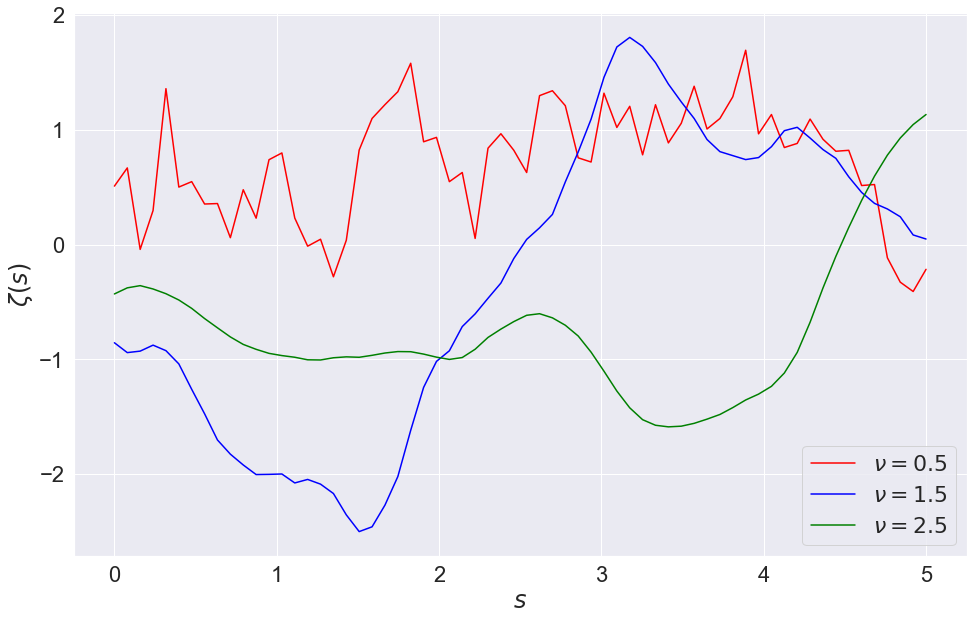
\includegraphics[width=1.0\textwidth]{example_kernel}
	\caption[Example realisations from a Gaussian processes with the Mat\'ern covariance function with differing $\nu$ parameters.]{Example realisations from Gaussian processes with the Mat\'ern covariance function with differing $\nu$ parameters. We plot a single realisation from each of three processes with $m(s) = 0$ and $k(s) = C_\nu(d(s, s^\prime))$ for $\nu = 0.5, 1.5, 2.5$ over the domain of $\mathcal{S} = \left[0, 5\right] \subset \mathbb{R}$.}
	\label{fig:example_matern}
\end{figure}

The issue with stationary covariance forms is that they are often quite restrictive in the sense that the correlation structure cannot vary across the domain.
For example, this might be a too restrictive assumption in the case of climate data where correlation structure might be quite different in different parts of the globe. 
One particular way to extend the stationary Mat\`{e}rn kernel to be non-stationary is proposed in \citep{paciorek_spatial_2006}.
\citeauthor{paciorek_spatial_2006} propose a method to knit together multiple stationary correlation functions such that the resultant function is non-stationary.

They provide a form of non-stationary covariance function $k^{NS}(\cdot, \cdot)$ from a stationary covariance  function $k^{S}(\cdot, \cdot)$ as follows, \citep{paciorek_spatial_2006}:
\begin{equation}\label{eqn:mat_ns}
	k^{NS}(\ve{s}, \vesup{s}{\prime}) = \lvert \Sigma_{\ve{s}} \rvert ^{\frac{1}{4}} \lvert \Sigma_{\vesup{s}{\prime}} \rvert^{\frac{1}{4}} \lvert \frac{ \Sigma_{\ve{s}}  + \Sigma_{\vesup{s}{\prime}}}{2}\rvert^{-\frac{1}{2}} k^S(Q(\ve{s}, \vesup{s}{\prime}))
\end{equation}
where $Q(\ve{s}, \vesup{s}{\prime}) = \left(\ve{s} - \vesup{s}{\prime}\right)^\transpose \left( \frac{ \Sigma_{\ve{s}}  + \Sigma_{\vesup{s}{\prime}}}{2}\right)^{-1}  \left(\ve{s} - \vesup{s}{\prime}\right)$ and $\Sigma_{\ve{s}} = \Sigma(\ve{s})$ is the covariance matrix of the Gaussian kernel centred at $\ve{s}$. How $\Sigma_{\ve{s}}$ varies across the domain specifies how non-stationary the full covariance kernel is.

There have been other proposed approaches for introducing non-stationarity into the kernels of Gaussian processes.
\citeauthor{sampson_nonparametric_1992} considers a non-parametric estimation procedure to model non-stationary kernels, \citep{sampson_nonparametric_1992}.
Whilst non-stationary kernels have been consider by combining locally stationary kernels, \cite{genton_classes_2001}.
Both of the above methods are interesting in their own right, however in this work we focus on the class of covariances formed through \citeauthor{paciorek_spatial_2006} methods; as described above.


With almost all covariance functions and especially non-stationary covariances there are typically hyper parameters which must be estimated from the data.
For example in the Mat\`{e}rn covariance we have the shape parameter $\nu$ and any length scale parameters defined in the distance function $d(\cdot, \cdot)$.
These are typically estimated though maximum likelihood estimation, \citep{williams_gaussian_2006}, however fully Bayesian estimation can also be achieved through some Markov Chain Monte Carlo (MCMC) scheme, \citep{paciorek_spatial_2006}. 